\documentclass{article}

\usepackage{graphicx}
\usepackage{subcaption}
\usepackage{amsmath}
\usepackage{amsfonts}

\begin{document}

\author{Zachary Vogel}
\date{\today}
\title{Notes in APPM 4650\\Adam Norris}

\maketitle

\section{Still doing project}
few remaining words about explosion problem.\\
In theory you have:\\
\[\frac{d\theta}{d\sigma}=\delta e^{\theta}-\theta\]
stiff problem.\\
\[\sigma_{\text{explosion}}=\int_0^\infty \frac{dx}{\delta e^x-x}\]
where infinity is big enugh so that the value of the integral doesn't change.\\

Thus, we have project 1.\\

\section{Project 2}

\begin{figure}[h!]
    \centering
    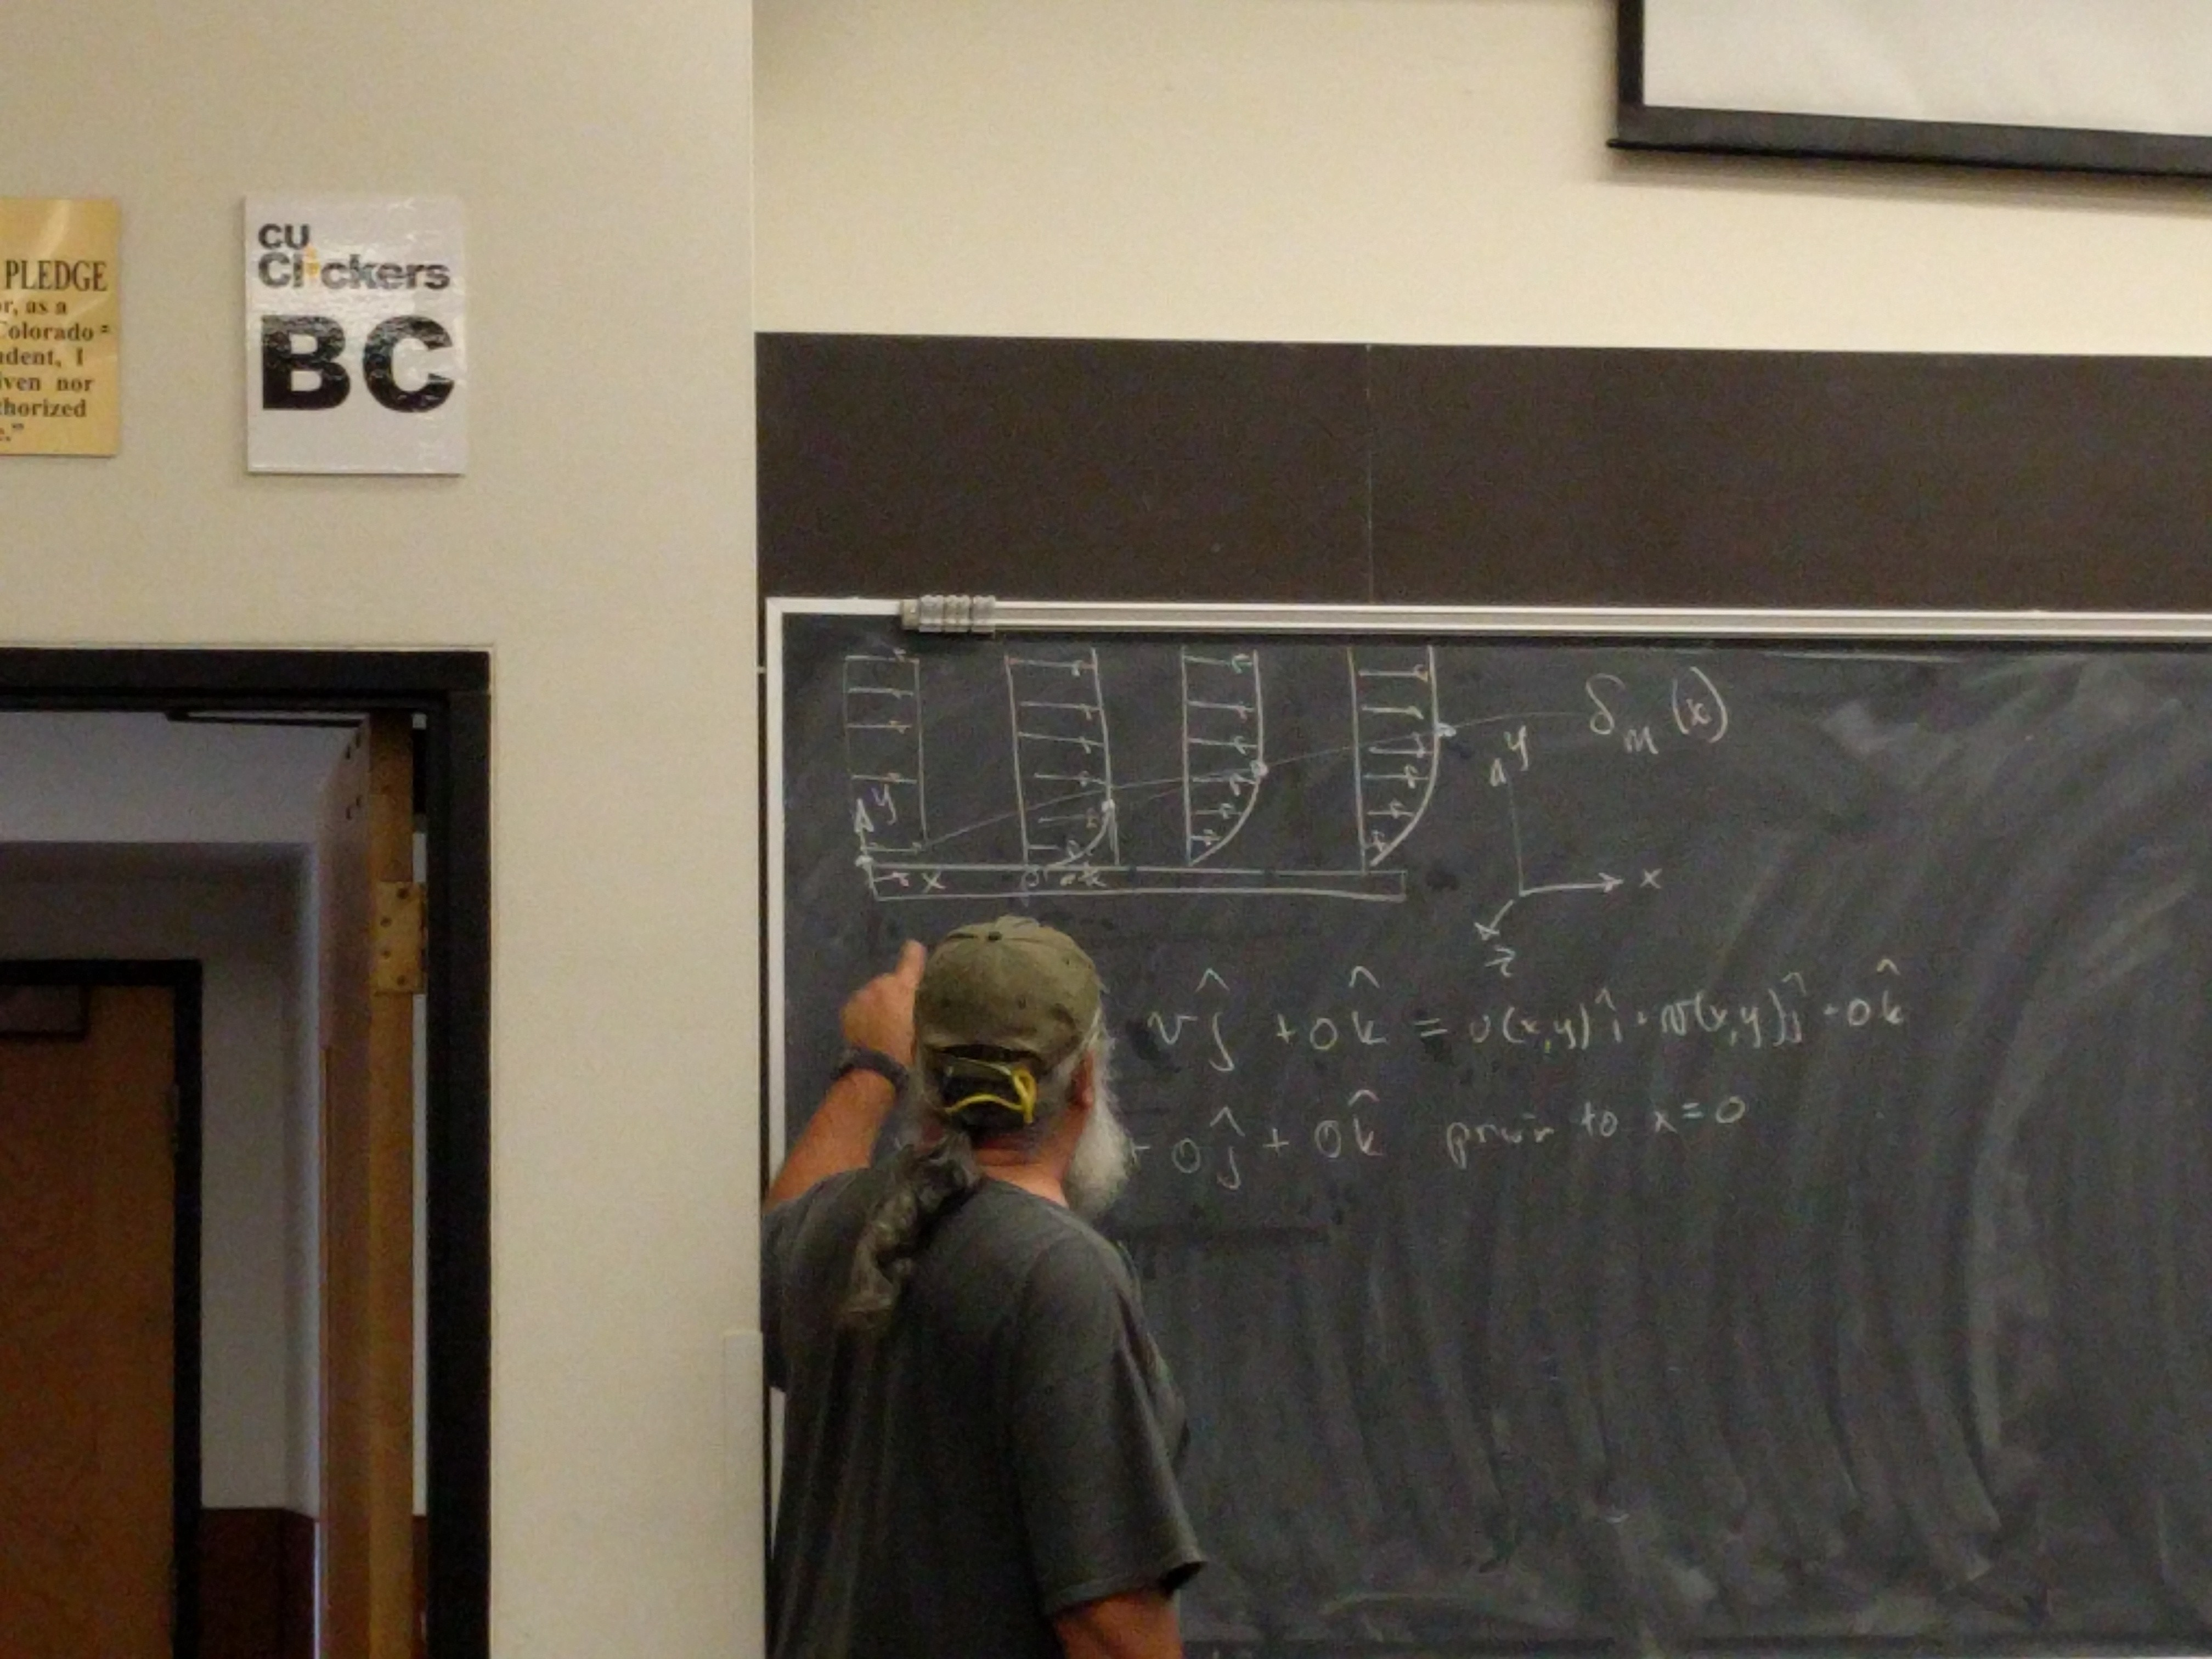
\includegraphics[clip=true,trim={45cm 45cm 45cm 40cm},width=0.8\textwidth]{flow1.jpg}
\end{figure}

fluid flowing from left to right, flowing at velocity of $u_{\infty}$.\\
generic velocity:\\
\[v=u\hat{i}+\mathfrak{v}\hat{j}+0\hat{k}=u(x,y)\hat{i}+\mathfrak{v}(x,y)\hat{j}+0\hat{k}\]
it's all horizontal as it approaches a flat plate.\\
when you first hit the plate:\\
\[v=u_{\infty}\hat{i}+0\hat{j}+0\hat{k}\]
prior to $x=0$.
$\delta_m(x)$ momentum boundary layer thickness.\\
goal is to find\\
$u(x,y)=\dots,\quad v(x,y)=\dots$\\

\begin{figure}[h!]
    \centering
    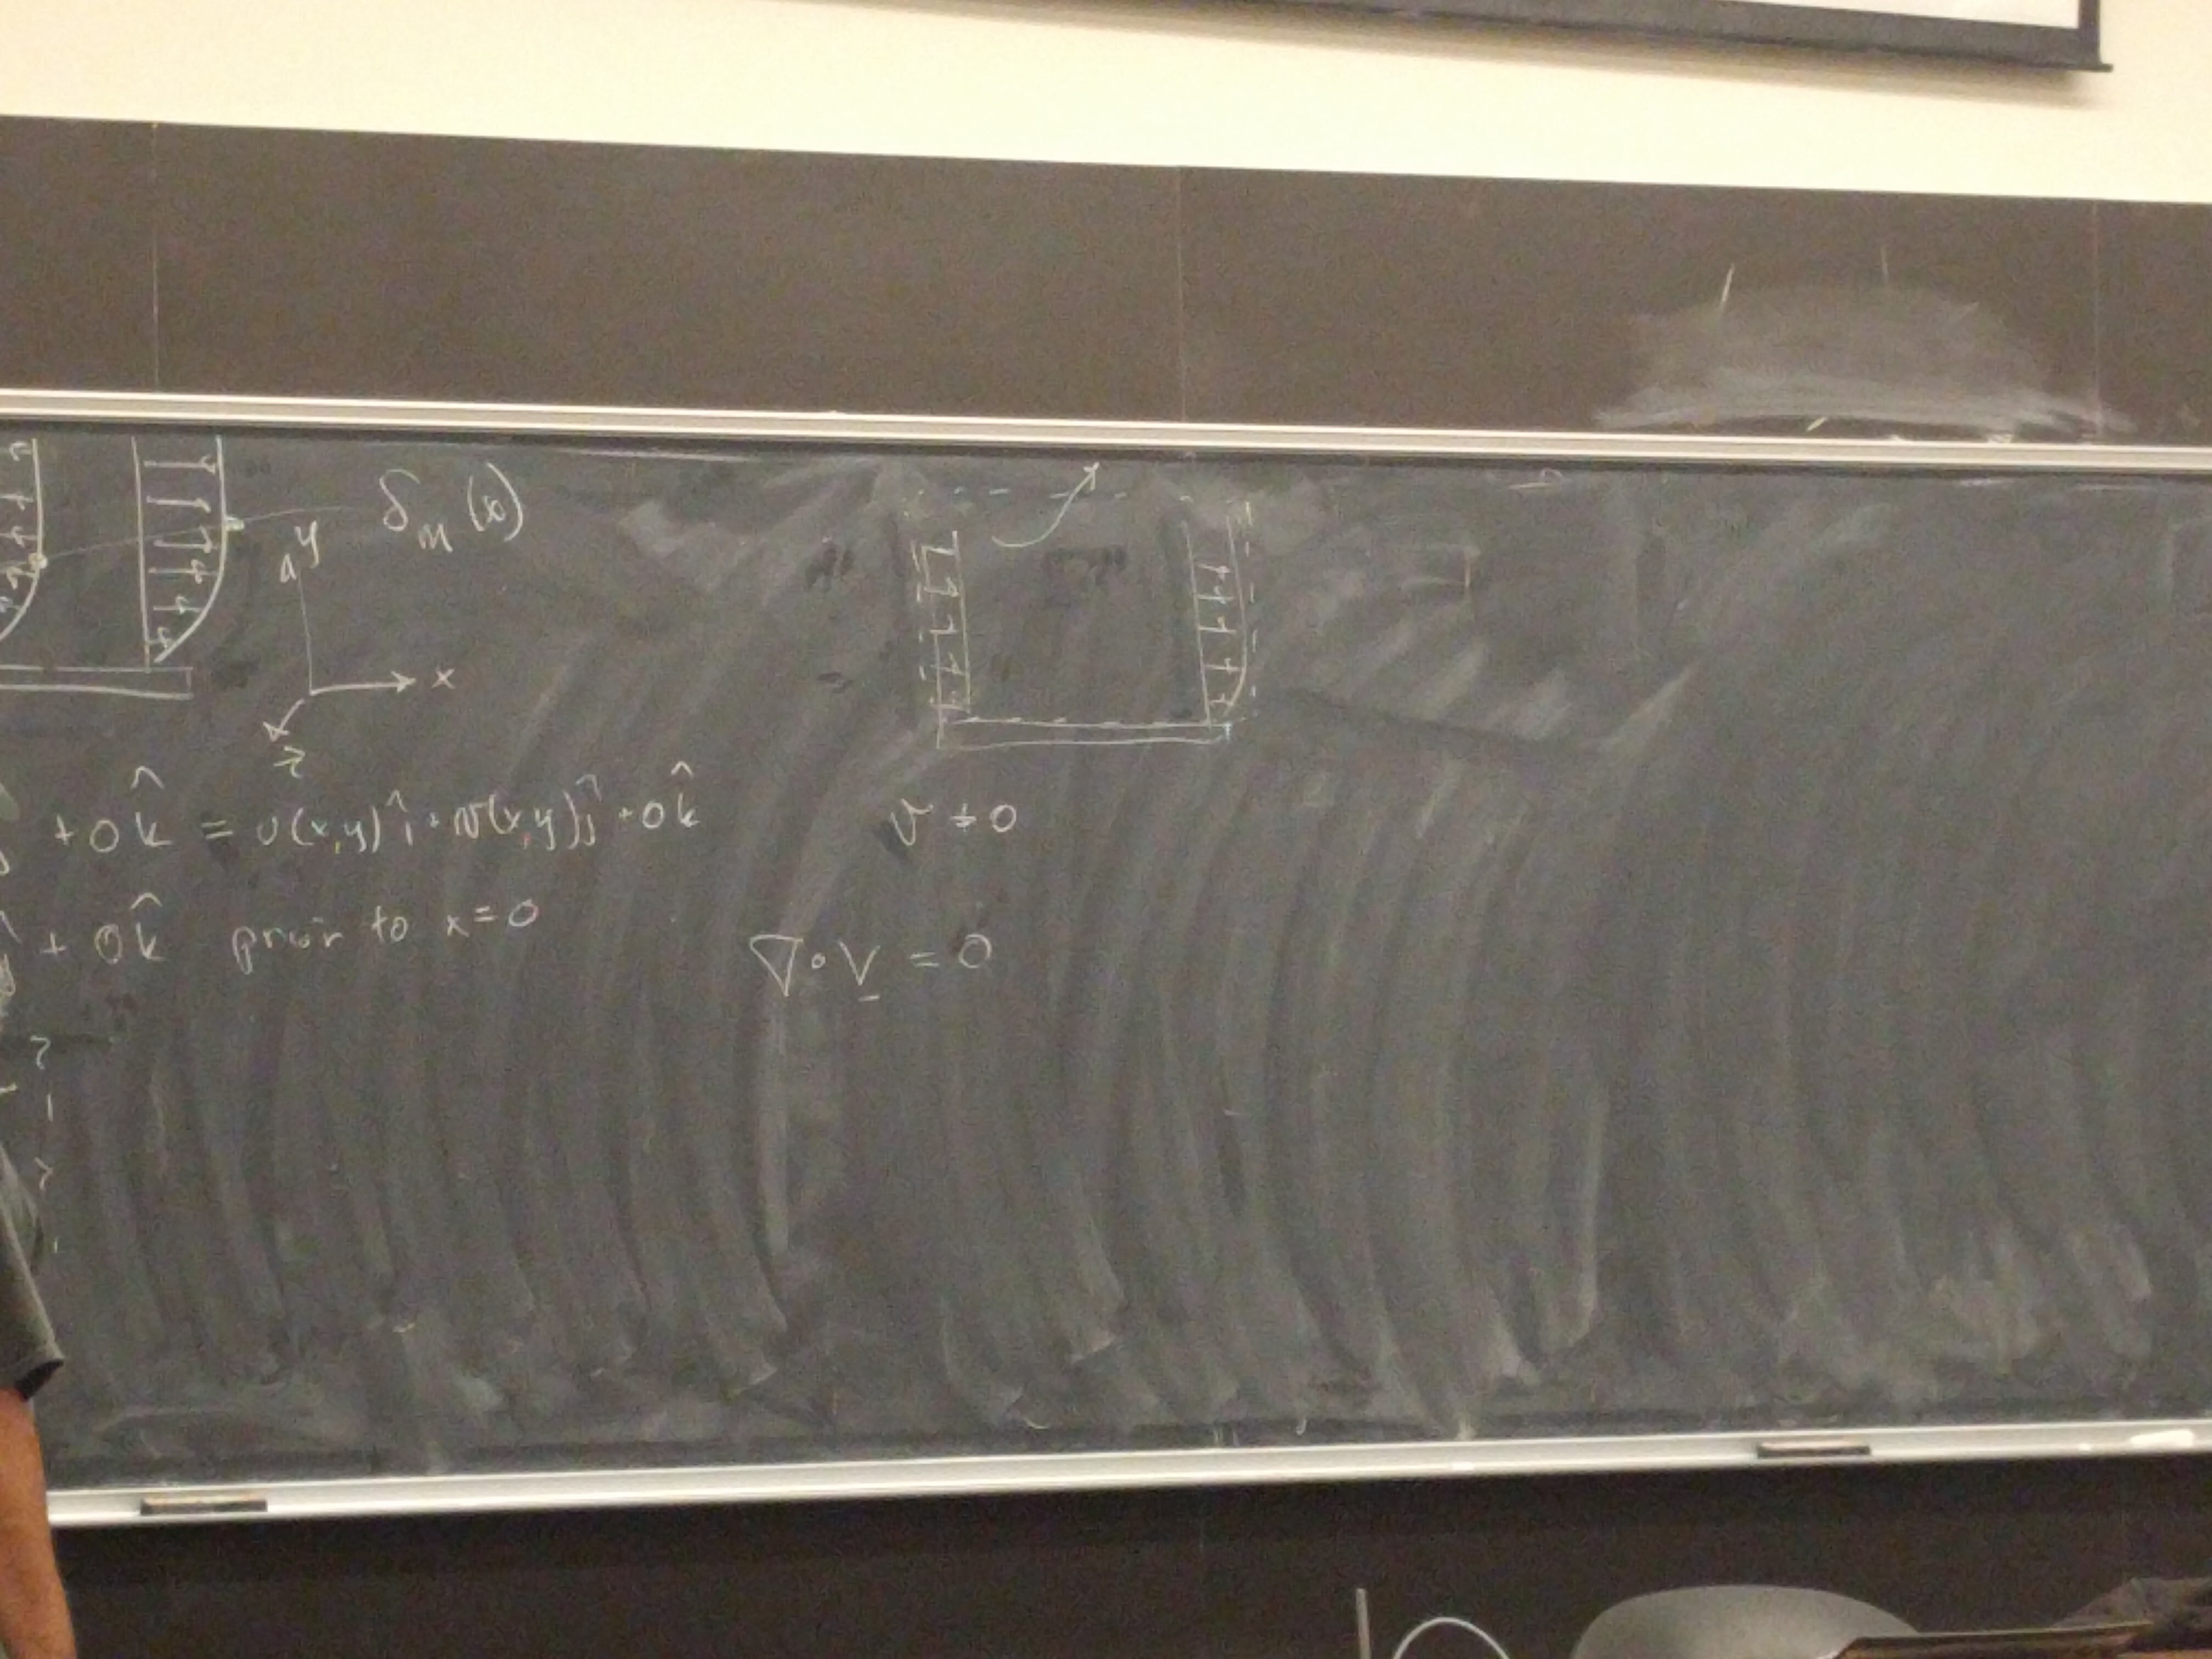
\includegraphics[clip=true,trim={45cm 56cm 45cm 30cm},width=0.8\textwidth]{flow2.jpg}
\end{figure}
divergence is the stuff coming out from every point.\\
$v\neq 0$\\
\[u_x+u_y=0\]
conservation of mass.\\

\[uu_x+\mathfrak{v}u_y=\nu u_{yy}\]
conservation of x momentum.\\
\[\frac{du}{dt}+(v_0\nabla) u=v\nabla^2 u\]
$\frac{du}{dt}$ is gone by s.s.\\

also, the plate is hot and the fluid is cold, so now we get to worry about that.\\
conservation of mass: $u_x+u_y=0$\\
conservation of momentum: $uu_x+\mathfrak{v}V_y=\nu u_{yy}$\\
$\nu\sim$ kinematic viscosity$=\frac{\mu}{\rho}$\\
$\mu\sim$ dynamic viscosity\\
$\rho\sim$ mass density $\frac{\text{mass}}{\text{velocity}}$.\\

temperature of different regions as they pass over the hot plate. The further down you go, the thicker the region that has been warmed up as you can see.\\
temp stays at relatively the same temperature.\\
ever growing thickness known as $\delta_T$ $\delta$ thermal.\\
There you make a transition from $T_\infty$ to $T_{\text{wall}}$.\\
Conservation of thermal energy:\\
\[U\frac{\partial T}{\partial x}+\mathfrak{v}\frac{\partial T}{\partial y}=\alpha \frac{\partial^2 T}{\partial y^2}\]
convection                    and thermal diffusion.\\
$\alpha=\frac{k}{\rho c_p}$ thermal diffusivity.\\
\begin{figure}[h!]
    \centering
    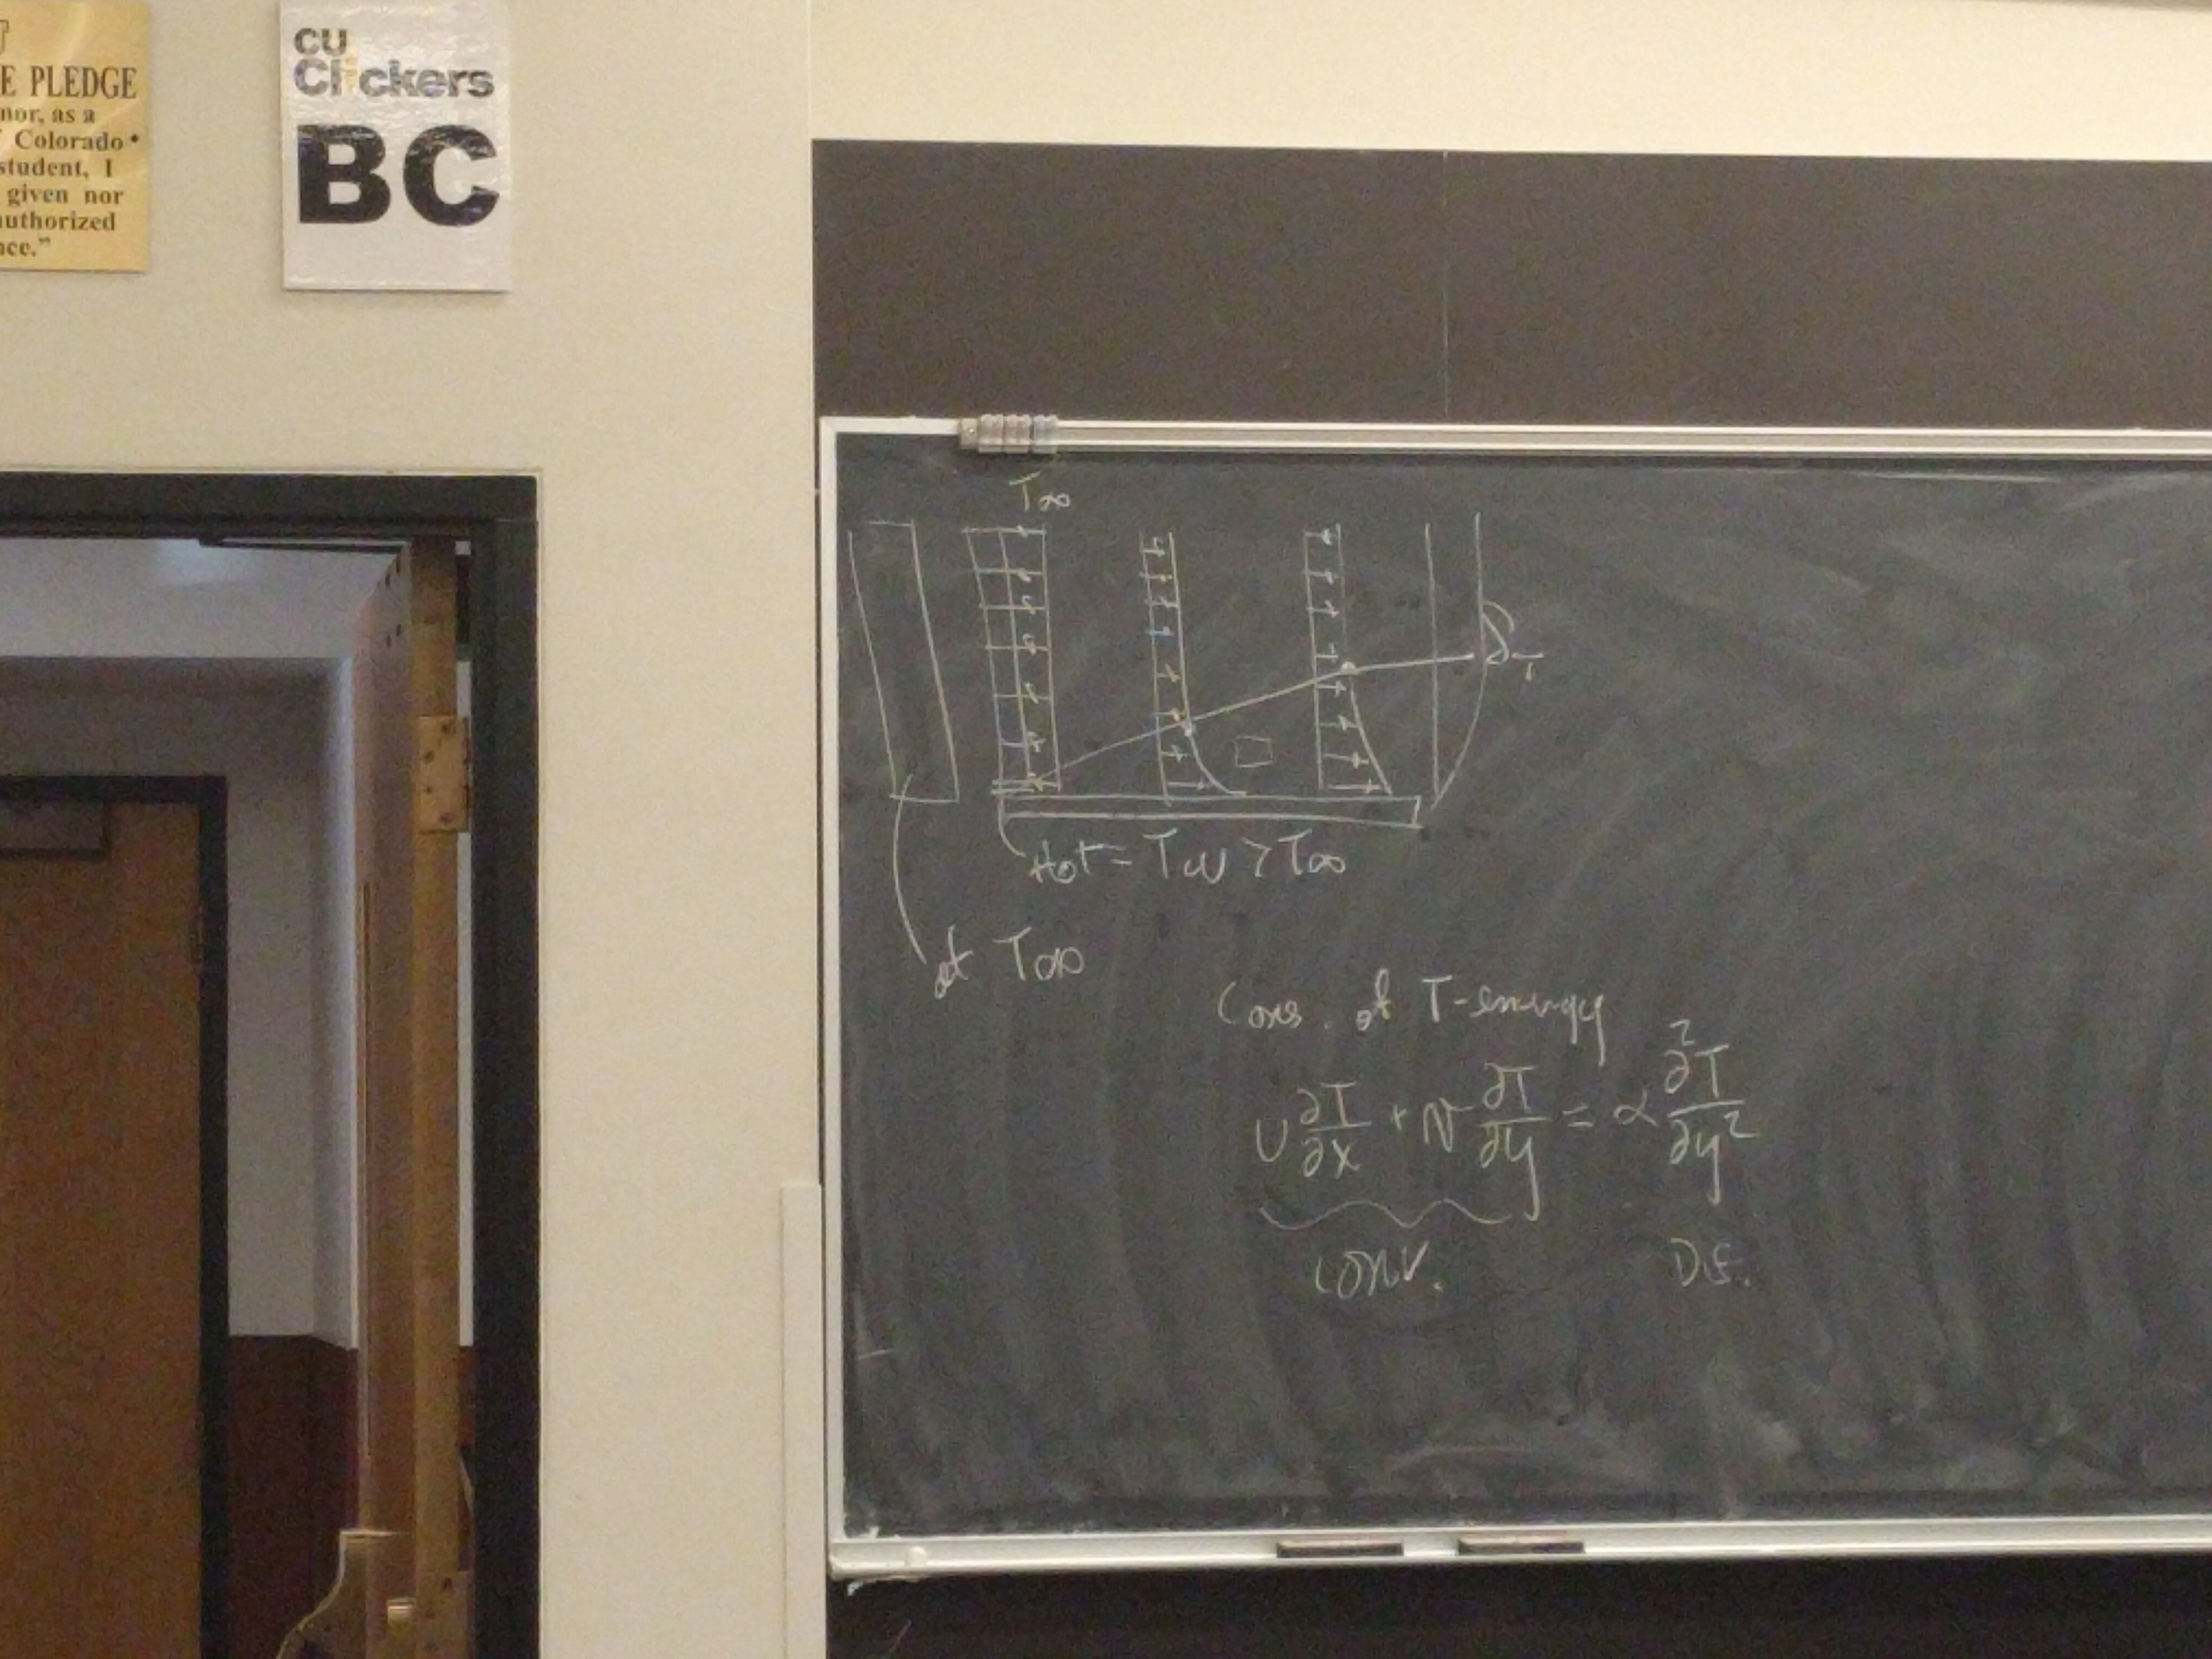
\includegraphics[clip=true,trim={50cm 40cm 33cm 30cm},width=0.8\textwidth]{flow3.jpg}
\end{figure}


\end{document}
